% 2011 Anhui science q21 fig1: parabola y=x^2, A=(1,1), B(-4/3,16/9), Q on AB, vertical through Q meets parabola at M, P below axis with QM=lambda*MP (lambda=3).
\usetikzlibrary{arrows.meta}
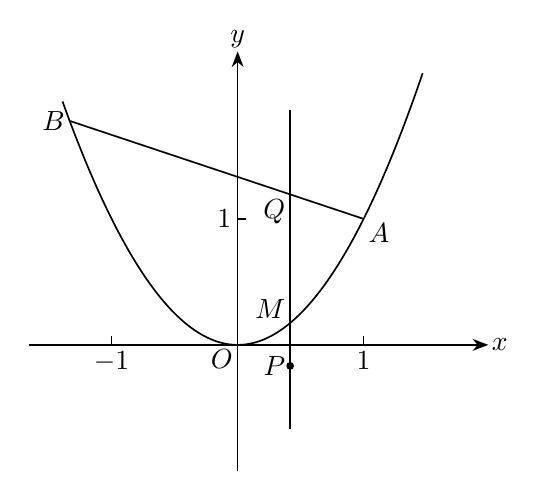
\begin{tikzpicture}[x=1.6cm,y=1.6cm,line width=.6pt,>=Stealth,font=\normalsize]
\coordinate (O) at (0,0);
\coordinate (A) at (1,1);
\coordinate (B) at (-1.333333333333,1.777777777778);
\coordinate (Q) at (0.416666666667,1.194444444444);
\coordinate (M) at (0.416666666667,0.173611111111);
\coordinate (P) at (0.416666666667,-0.166666666667);
\coordinate (Xl) at (-1.66,0);
\coordinate (Xr) at (1.99,0);
\coordinate (Yd) at (0,-1.0);
\coordinate (Yu) at (0,2.33);
\coordinate (Vtop) at (0.4166667,1.867);
\coordinate (Vbot) at (0.4166667,-0.664);
% parabola y = x^2
\draw[domain=-1.39:1.47,samples=141,variable=\t] plot ({\t},{\t*\t});
% axes
\draw[->] (Xl)--(Xr) node[right,inner sep=1pt] {$x$};
\draw[->] (Yd)--(Yu) node[above,inner sep=1pt] {$y$};
% axis ticks
\draw (-1,0)--(-1,0.07);
\draw (1,0)--(1,0.07);
\draw (0,1)--(0.07,1);
\node[below,inner sep=2pt] at (-1,0) {$-1$};
\node[below,inner sep=2pt] at (1,0) {$1$};
\node[left,inner sep=2pt] at (0,1) {$1$};
% line AB
\draw (B)--(A);
% vertical line through Q
\draw (Vbot)--(Vtop);
% point P (filled)
\fill (P) circle (1.4pt);
% labels
\node[below left,inner sep=1.5pt] at (O) {$O$};
\node[below right,inner sep=1.5pt] at (A) {$A$};
\node[left,inner sep=1.5pt] at (B) {$B$};
\node[below left,inner sep=1.5pt] at (Q) {$Q$};
\node[above left,inner sep=1.5pt] at (M) {$M$};
\node[left,inner sep=1.5pt] at (P) {$P$};
\end{tikzpicture}
